\chapter{Introducción Específica} % Main chapter title

\label{Chapter2}

%----------------------------------------------------------------------------------------
%	SECTION 1
%----------------------------------------------------------------------------------------
En este capítulo se presenta los componentes de CIAABOT, con un poco más
de detalle, se analiza una alternativa real para depuración y se justifica el diseño
propuesto de \emph{debugging} a implementar, luego se establecen los requerimientos y
la planificación para el desarrollo del presente trabajo.

\section{Componentes CIAABOT}
\label{sec:Componentes CIAABOT}
La plataforma esta conformada por tres partes fundamentales, tal como se muestra en la figura \ref{fig:componentesCiaabot}. 

A continuación se describirá en detalle cada una de las partes de CIAABOT.

\begin{figure}[h]
	\centering
	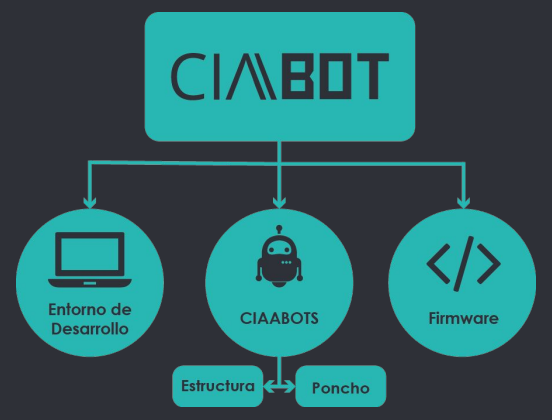
\includegraphics[scale=.50]{./Figures/componentesCiabot.png}
	\caption{Componentes CIAABOT. Recuperado de \url{https://laboratorios.fi.uba.ar}}
	\label{fig:componentesCiaabot}
\end{figure}

\subsection{CIAABOT IDE}

El IDE esta basado en el paradigma reactivo que permite armar programas propios, que pueden ser programas puntuales como manejo de actuadores y motores
en un sistema embebido, así como también, un prototipado rápido.

El IDE de CIAABOT tiene como componente principal al editor, a partir de allí el usuario puede empezar a desarrollar su propio programa gráfico encastrando de manera fácil bloques predifinidos creado en lenguaje javascript, como se observa en la figura \ref{fig:ciaabot-ide-bloques} 

El entorno de desarrollo integrado está diseñado para crear programas de forma sencilla encastrando bloques gráficos. Asimismo, permite de manera gradual ir comprendiendo como realizar el mismo programa en lenguaje C, debido a que permite ver en tiempo real el código C generado mientras se van encastrando los bloques.

Dentro del entorno se brinda al usuario, una barra de herramientas con funcionalidades
para crear un nuevo programa, compilarlo, y realizar la descarga del
código en la placa conectándola por USB.

El IDE proporciona al usuario la opción de guardar el programa creado en un
archivo con extensión .cbp, el cual contiene toda la información del programa
creado, que podría ser utilizado posteriormente. 

\begin{figure}[h]
	\centering
	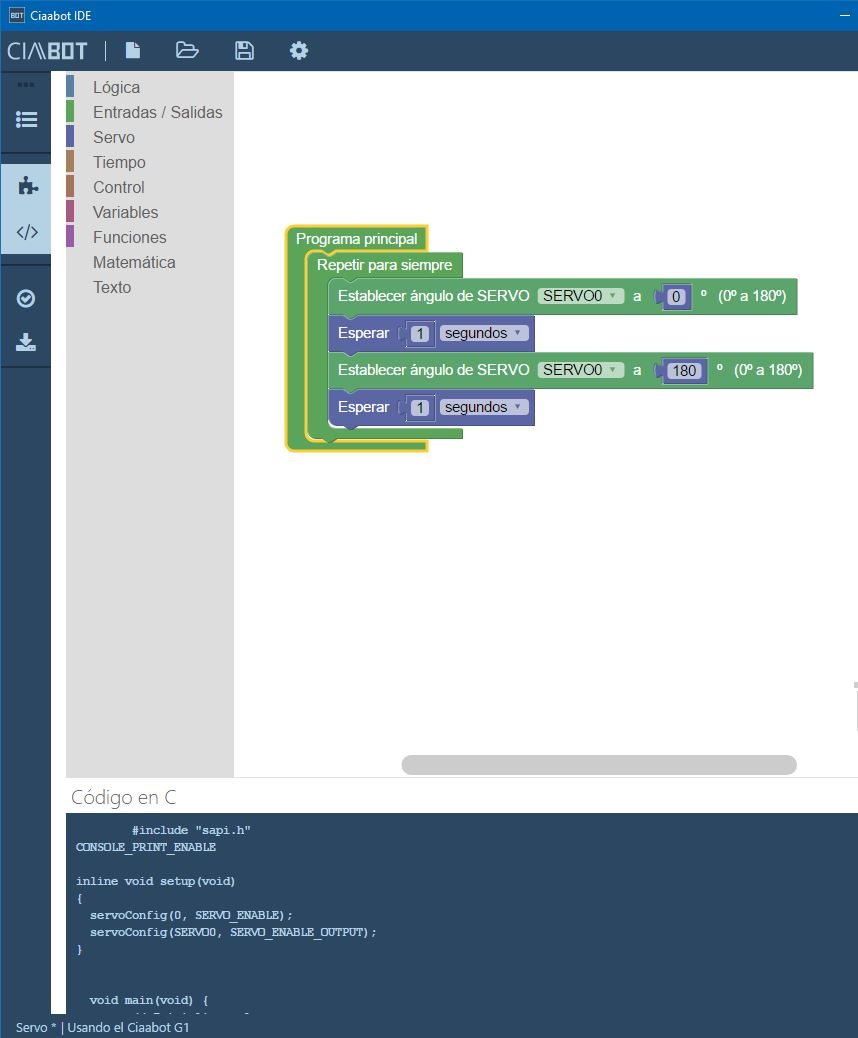
\includegraphics[scale=.30]{./Figures/ciaabot-ide-bloques.JPG}
	\caption{Editor gráfico de CIAABOT-IDE.}
	\label{fig:ciaabot-ide-bloques}
\end{figure}

La plataforma CIAABOT esta programado usando las siguientes tecnologías:

\begin{itemize}
	\item Angular\citep{angular}.
	\item Blockly\citep{blockly}.
	\item Electrón\citep{electron}.
	\item NodeJS\citep{nodejs}.
	\item TypeScript\citep{typescript}
\end{itemize}

El funcionamiento principal en la plataforma CIAABOT es la siguiente:

\begin{itemize}
	\item Genera el archivo principal: archivo main.c
	\item Genera el código en C: cada uno de los bloque genera el correspondiente codigo en C y lo inyecta en el archivo main.c del programa.
	\item Permite la ejecución del compilador de C para el código en la placa.
	Invoca al OpenOCD.
	\item Descarga el binario compilado en flash y realiza el reset.
\end{itemize}

\subsection{CIAABOTS}
\label{subsec:CIAABOTS}

La plataforma usa CIAABOTS para llamar así a los robots que se pueden programar utilizando CIAABOT IDE. Estos CIAABOTS tienen un diseño estructural de impresión en 3D, correspondiente al modelo de la placa CIAA. 

Para ser usados por las impresoras 3D, es necesario armar el poncho de diseño abierto y tener los sensores y actuadores del CIAABOT a imprimir.

\subsection{Firmware}
\label{subsec:Firmware}

Debido a que la plataforma CIAABOT esta basado en el firmware v2 \citep{CIAA:firmwarev2} del proyecto CIAA, puede crear desde funciones simples a más complejas, para realizarlo
utiliza las siguientes herramientas:

\begin{itemize}
	\item \emph{Makefile}: para la gestión de dependencias, de esta manera puede construir
	el software desde sus archivos fuente.	
	\item \emph{OpenOCD}: una herramienta OpenSource, usado para el grabado del firmware
	en las placas.
	\item \emph{sAPI}\citep{sAPI}: permite manejar los periféricos del microcontrolador de una manera
	muy sencilla.
\end{itemize}


\section{Alternativas de diseño para CIAABOT debugger}
\label{sec:Alternativas de diseño para CIAABOT debugger}

Para diseñar el software de depuración se toma como caso de estudio, la depuración de un programa en lenguaje C mediante Eclipse IDE:

\begin{itemize}
	\item \emph{Plugin de eclipse arm-none-eabi-gdb}
	\footnote{Software de configuración de eclipse para usar el depurador GNU para procesadores ARM Cortex-A/R/M.}: realiza la interpretación de comandos de	GDB-MI y muestra los resultados en la interfaz gráfica del editor de texto de C en el IDE del Eclipse.
	\item \emph{arm-none-eabi-gdb}
	\footnote{Software de debug originario de linux.}: realiza el mapeo de los símbolos de C con las instrucciones en código máquina que se ejecutan en el microcontrolador (mapea las funciones al código binario en flash), para
	luego ejecutar los comandos de parar, continuar o de uso de brakpoints. Se podría debuggear también, por línea de comandos directamente sobre el código C abriendo GDB en una terminal con comandos GDB-MI y usando los archivos .elf y .bin generados.
	\item \emph{OpenOCD (Open On-Chip Debugger)}\footnote{Software de código abierto que interactúa con el puerto JTAG de un depurador de hardware.}: prevee a GDB el remote interface protocol para permitirle acceder al hardware. Traduce transacciones JTAG o SWD (mediante el puerto serie sobre USB) a comandos remote-protocol de GDB. OpenOCD utiliza scripts de configuración (archivos *.cfg) donde se describe el microcontrolador a depurar y la interfaz de hardware para acceder al mismo (en adelante \emph{"Debugger HW"}).
	\item \emph{Debugger (HW)}: en el caso de la EDU-CIAA es la placa de interfaz fisica para pasar de JTAG a USB (modo puerto serie virtual). En la EDU-CIAA
	viene incluido en la misma placa que esta el micro y usa todo el circuito de hardware para debug.
	\item \emph{Microcontrolador a debuggear}: El microcontrolador posee un periferico específico para \emph{debug} con interfaz JTAG
	\footnote{Acrónimo de Joint Test Action Group, es utilizado como mecanismo para depuración de sistemas embebidos, proveendo una puerta trasera para acceder al sistema.}, teniendo acceso para modificar la RAM, Flash (externas al microcontrolador) y los registros del Microcontrolador.
\end{itemize}

Una alternativa para la programación de un software de depuración a nivel de bloques de CIAABOT es, entonces, mantener el mapeo entre los bloques de programa de CIAABOT y su C generado y comunicarse con GDB, mediante GDB-MI como lo realiza el plugin de Eclipse.

Teniendo en cuenta la complejidad de implementar lo visto anteriormente, se propone como una alternativa factible, el de emular la funcionalidad de debugger mediante la ejecución del programa de CIAABOT en la propia PC, de manera que al momento de ejecutarse los bloques gráficos de acceso a los periféricos, se realice la comunicación con la placa mediante un protocolo, y de esta manera realizar la ejecución de comandos de lectura y escritura en los periféricos que se quiere manipular.

Debido a que existe como antecedente el proyecto firmata4CIAA se decidió utilizarlo como protocolo para acceso al Hardware.


\section{Firmata}
\label{sec:Firmata}

Firmata es un protocolo genérico para comunicarse con microcontroladores desde
el software en una computadora (o teléfono inteligente / tableta, etc.).

Este protocolo fue diseñado para la comunicación directa entre un microcontrolador y un objeto de software en una computadora host Cliente Firmata. En la figura \ref{fig:componentesFirmata} se muestra la Arquitectura de este protocolo.

Firmata4CIAA es un programa que implementa el protocolo firmata en la EDU-CIAA-NXP.

\begin{figure}[h]
	\centering
	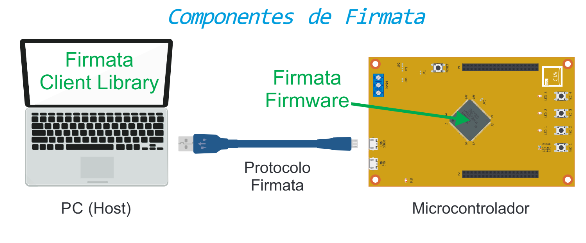
\includegraphics[scale=.80]{./Figures/componentesFirmata.png}
	\caption{Arquitectura de Firmata.}
	\label{fig:componentesFirmata}
\end{figure}

\subsection{Johnny-Five}
\label{subsec:Johnny-Five}

Cliente firmata, basado en el lenguaje JavaScript. Es un marco de programación de fuente
abierta, basado en el protocolo firmata, IoT y Robótica. En la figura \ref{fig:johnny} se presenta a este framework.

\begin{figure}[h]
	\centering
	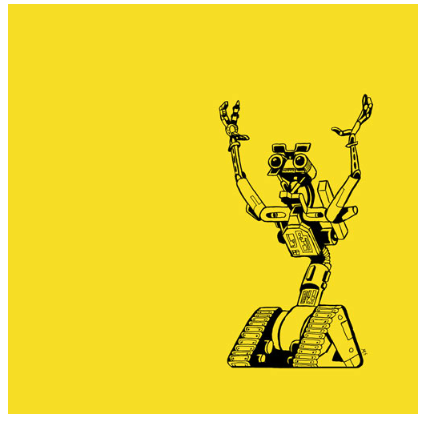
\includegraphics[scale=.50]{./Figures/johnny.png}
	\caption{Cliente firmata: Johnny-Five. Recuperado de \url{http//johnny-five.io}} 
	\label{fig:johnny}
\end{figure}

De esta manera se propone la comunicación entre la aplicación y la placa EDUCIAA-NXP.

\section{Sistema para depuración propuesto}

Después de lo visto en las secciones anteriores, se propone el siguiente sistema a diseñar:

\begin{itemize}
	\item Ejecutar un programa línea a línea, que ejecute los bloques en javascript en la PC del usuario..	
	\item Enviar comandos firmata a la placa, solo cuando se encuentre un bloque de acceso a algún periférico.
	\item Visualizar el contenido de las variables en un determinado momento de la ejecución.
	\item Instalación del protocolo firmata de la CIAA, sólo en el caso de ser necesario.
	\item Entorno gráfico amigable.
\end{itemize}

\subsection{Limitación}
\label{subsec:Limitación}

En este sistema propuesto, existen dos tipos de ejecución de bloques:

\begin{itemize}
	\item Bloques gráficos que acceden a los periféricos: son aquellos que usarán el protocolo firmata para enviar comandos a la placa, y mediante las funciones por UART se van comunicando con el hardware. Por ejemplo en el manejo de sensores, motores, etc.
	\item Bloques gráficos que no acceden a los periféricos: son aquellos que se ejecutan en la misma pc, por medio de javascript. Por ejemplo las sentencias loop-for, if-else, etc.
\end{itemize}

Los bloques gráficos que acceden a los periféricos, en tiempo de acceso de ejecución,
serán más lentos que si se tuviera que implentar la alternativa de diseño de
la sección \ref{sec:Alternativas de diseño para CIAABOT debugger}, ya que ese programa accedería al hardware a la velocidad en la que
se llama a las instrucciones del hardware, debido al código binario compilado
instalado en la placa.

Por el contrario, los bloques gráficos que no acceden a los periféricos, en tiempo
de ejecución, serán más rápidos, debido a que se ejecutarán directamente en la
misma PC del usuario. El programa se ejecutará dentro del contexto del VM de
javascript, que es más rápido que el código c compilado en el microcontrolador.

En conclusion si medimos los tiempos de ensayos, cuando se instala el firmware
del codigo C generado en la placa contra la ejecución de los bloques con firmata, estos tiempos no serán los mismos.

\subsection{Ventaja}
\label{subsec:Ventaja}

Para el usuario de CIAABOT, este método será una ventaja, ya que podrá depurar el programa sin necesidad de esperar la generación del código C a partir del programa en bloques, su compilación (especialmente en Windows) y descarga a la plataforma.

\section{Requerimientos}
\label{sec:ejemplo}

Se plantearon requerimientos que el proyecto debe cumplir a la hora de ser en-
tregado. Se evaluaron sus posibilidades y se clasificaron en categorías.

\subsection{Requerimientos asociados con el Proyecto CIAABOT}

\begin{itemize}
	\item El entorno de programación deberá poder ejecutarse minimamente dentro del entorno Linux y Windows.	
	\item El uso debe ser sencillo, rápido e intuitivo.
	\item El entorno de debugger debe tener un diseño basado en ventanas cómodas y que permitan
	tener mucha información a la vista.
	\item El entorno de debugger debe ocupar muy poca memoria.
	\item El diseño de la herramienta debe seguir los estilos de interfaz establecidos en el Proyecto CIAABOT.
	\item La herramienta debe poder permitir el monitoreo de las entradas y salidas de los diferentes periféricos de la placa.	
\end{itemize}

\subsection{Componentes establecidos en CIAABOT}

\begin{itemize}
	\item El presente proyecto deberá integrarse al entorno gráfico establecido que permita la programación de los robots.	
	\item Se usará la placa EDU-CIAA-NXP (figura \ref{fig:edu-ciaa-nxp}) para el control de los robots.	
\end{itemize}

\begin{figure}[h]
	\centering
	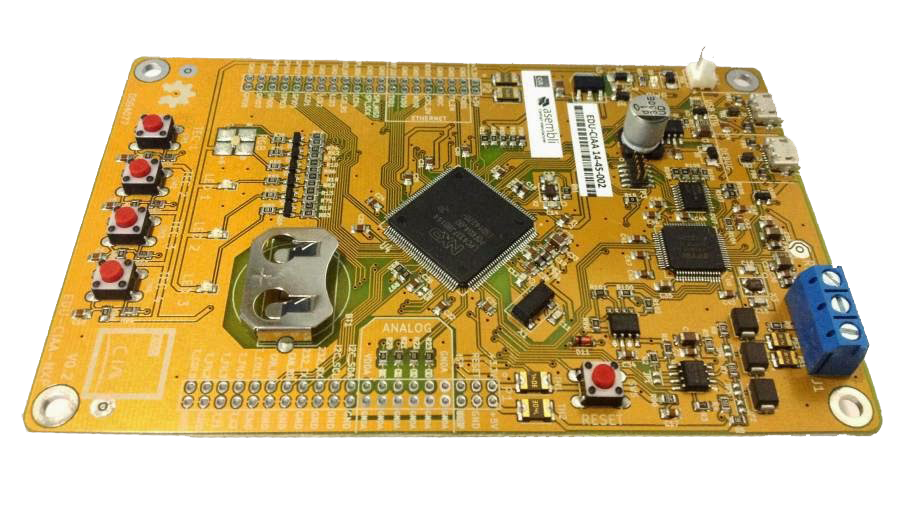
\includegraphics[scale=.30]{./Figures/edu-ciaa-nxp.png}
	\caption{Placa EDU-CIAA-NXP}
	\label{fig:edu-ciaa-nxp}
\end{figure}

\subsection{Firmware}

\begin{itemize}
	\item Se actualizará a la última versión, respetando el control de versiones establecido.	
	\item Se utilizarán las principales bibliotecas firmata que permita interactuar con el cliente que está corriendo en la placa.
	\item Se contará con un mecanismos de ahorro de la flash, para saber si la placa ya tiene firmata.
\end{itemize}

\subsection{Procesos Finales}

\begin{itemize}
	\item Se actualizará el manual de usuario, y se incluirán ejemplos básicos funcionales del entorno de depuración.	
	\item Se utilizarán las principales bibliotecas firmata que permita interactuar con el cliente que está corriendo en la placa.
	\item Se implementará el debugger de la aplicación sobre una maqueta o robot adaptado a funcionar con la placa EDU-CIAA.
	\item Se evaluarán los resultados del proyecto y su facilidad de uso en ámbitos de enseñanza reales.
\end{itemize}

\section{Planificación}
\label{sec:ejemplo}

Para lograr los objetivos propuestos, se realiza el desglose en tareas, y se utiliza las herramientas del diagrama de Activity on-node y gantt donde se esquematiza esas tareas que son parte del trabajo.

\subsection{Desglose en tareas} 

Para alcanzar objetivos concretos, se plantean los entragables para el proyecto:

\begin{itemize}
	\item Pluggin Debugger	
	\item Código fuente del proyecto debugger.
	\item Actualización del Manual de usuario, mostrando ejemplos didácticos del uso del debugger en la plataforma..
	\item El presente informe final.
\end{itemize}

Se estimó un tiempo aproximado de 600 horas, distribuidas en grupos de tareas de
la siguiente manera:

\begin{enumerate}
	\item Planificación del proyecto (60 hs.).
	
	\begin{itemize}
		\item Plan del proyecto.
		\item Análisis de requerimientos.
		\item Análisis técnico y de factibilidad.
		\item Gestión de riesgos.
		\item Gestión de calidad.
	\end{itemize}

	\item Investigación Preliminar (40 hs.).
	
	\begin{itemize}
		\item Búsqueda de plataformas de robótica educativa existentes, que en su interfaz de desarrollo implemente la herramienta de debugging.
		\item Búsqueda de frameworks de JavaScript, para la implementación de las funciones de firmata.
		\item Búsqueda de información acerca de la ejecución de debugging multiplataforma.
		\item Búsqueda de intérpretes Javascript para el debugging.
		\item Búsqueda de información de mecanismos de ahorro de la flash.
	\end{itemize}

	\item Selección de Frameworks (35 hs.).
	
	\begin{itemize}
		\item Selección y pruebas preliminares de la biblioteca firmata para JavaScript.
		\item Selección y pruebas preliminares del intérprete Javascript.
		\item Búsqueda de información acerca de la ejecución de debugging multiplataforma.
		\item Selección y pruebas del mecanismo de ahorro de la flash.
		\item Evaluar la correcta integración entre la aplicación CIAABOT y el debugger.
	\end{itemize}
	
	\item Desarrollo del Debugger (85 hs.).
	
	\begin{itemize}
		\item Desarrollo de estructura amigable e intuitiva para su uso.
		\item Desarrollo de estilos de componente compatibles a la aplicación CIAABOT.
		\item Desarrollo de módulo de configuración de mensajes al moverse los diferentes periféricos de la placa.
		\item Desarrollo del mecanismo de ahorro de la flash.
	\end{itemize}
	
	\item Implementaciones de funciones firmata javascript (90 hs.).
	
	\begin{itemize}
		\item Implementar los módulos para JavaScript encargados de obtener datos de cada sensor.
		\item Implementar los módulos para JavaScript encargados de manejar los actuadores.
		\item Desarrollo de funciones complementarias utilizando la API de JS Interpreter.
		\item Integración de las bibliotecas de programación gráfica.
	\end{itemize}

	\item Programación por Interfaz serie y Monitoreo Firmata (40 hs.).
	
	\begin{itemize}
		\item Desarrollo para mostrar mensajes en la interacción de los diferentes periféricos de la placa cuando está conectada por interfaz serie.
		\item Desarrollo de monitoreo en modo debug, de los estados de entradas y salidas a traves de firmata con visualización en la aplicación.
	\end{itemize}

	\item Pruebas de Firmware (60 hs.).
	
	\begin{itemize}
		\item Pruebas Unitarias.
		\item Pruebas de Integración.
		\item Corrección de errores encontrados.
	\end{itemize}

	\item Integración del Sistema (60 hs.).
	
	\begin{itemize}
		\item Integración de la aplicación Ciaabot para el modo debug.
		\item Pruebas iniciales de todo el sistema Ciaabot.
		\item Corrección de errores encontrados.
	\end{itemize}

	\item Procesos Finales (130 hs.).
	
	\begin{itemize}
		\item Modificar el manual de usuario, agregando el uso del modo debug.
		\item Redacción de memoria de trabajo.
		\item Evaluar el cumplimiento de requerimientos.
		\item Preparación de la presentación del proyecto.
	\end{itemize}

\end{enumerate}

\subsection{Activity On-node} 

En el diagrama de Activity on node de la figura  \ref{fig:diagramaNode} se muestran todas las tareas propuestas que se planificaron para realizar el proyecto, junto con su respectivo tiempo estimado en días para cada tarea.
Todas las flechas entrantes a un nodo o tarea son las dependencias de la misma.
 

\begin{figure}[h]
	\centering
	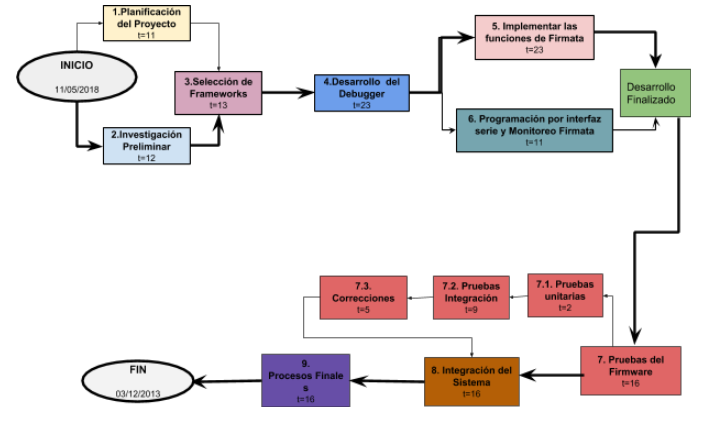
\includegraphics[scale=.60]{./Figures/diagramaNode.png}
	\caption{Diagrama de Node.}
	\label{fig:diagramaNode}
\end{figure}

Los días están expresados en días laborales de aproximadamente 3 horas, y en días no laborales de aproximadamente 4 horas. 
A modo de referencia se muestra en la siguiente figura  \ref{fig:tablaColores} una tabla de colores que se corresponde con cada una de las tareas.

\begin{figure}[h]
	\centering
	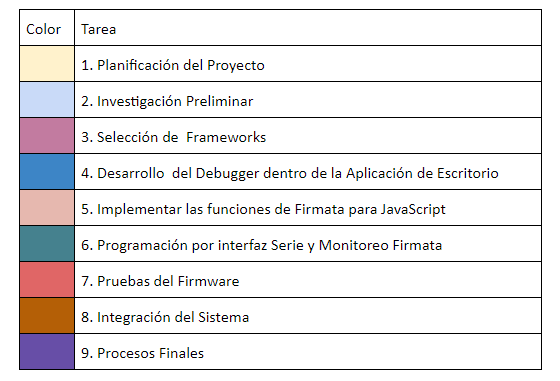
\includegraphics[scale=.60]{./Figures/tablaColores.png}
	\caption{Tabla de colores diagrama Activity}
	\label{fig:tablaColores}
\end{figure}

\subsection{Diagrama de Gantt}

El diagrama de Gantt permite tener una referencia rápida de dónde se debería encontrar el desarrollo del proyecto según la planificación inicial.
Por lo tanto, como parte de la planificación del proyecto, se definieron las tareas necesarias para completar el trabajo y se establecieron las relaciones de correlatividad entre ellas, teniendo en cuenta su duración. 

En la figura \ref{fig:diagramaGanttPrimeraParte} se puede observar la primera parte del diagrama para este proyecto. Las horas en la duración de cada una de las tareas están expresadas en días laborables y no laborables.

\begin{figure}[h]
	\centering
	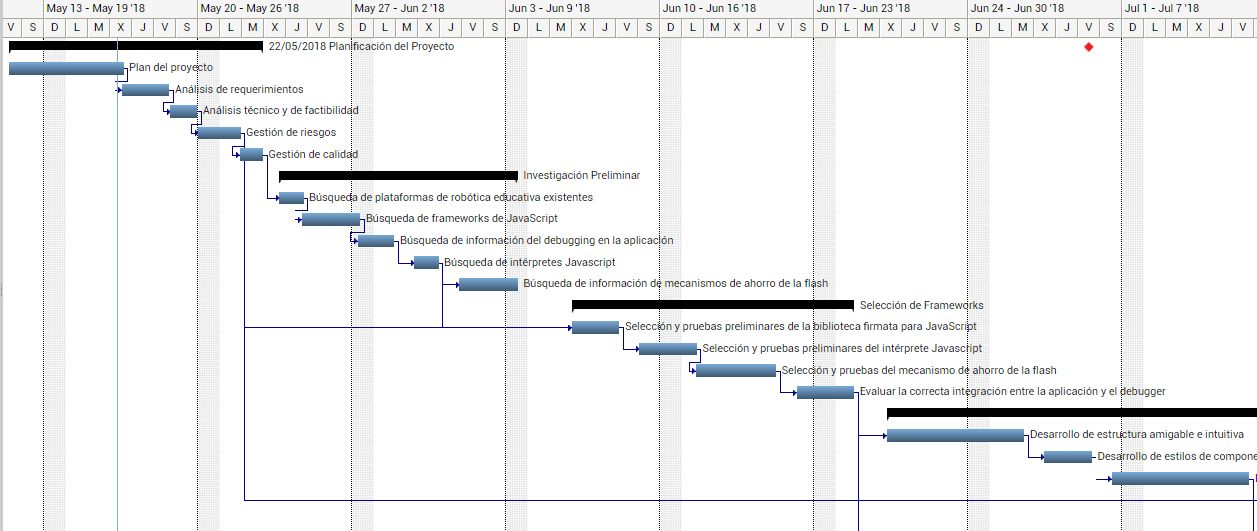
\includegraphics[scale=.30]{./Figures/diagramaGanttPrimeraParte.png}
	\caption{Diagrama de Gantt - Parte 1.}
	\label{fig:diagramaGanttPrimeraParte}
\end{figure}

En la figura \ref{fig:diagramaGanttSegundaParte} se puede observar la segunda parte del diagrama para este proyecto. 

\begin{figure}[h]
	\centering
	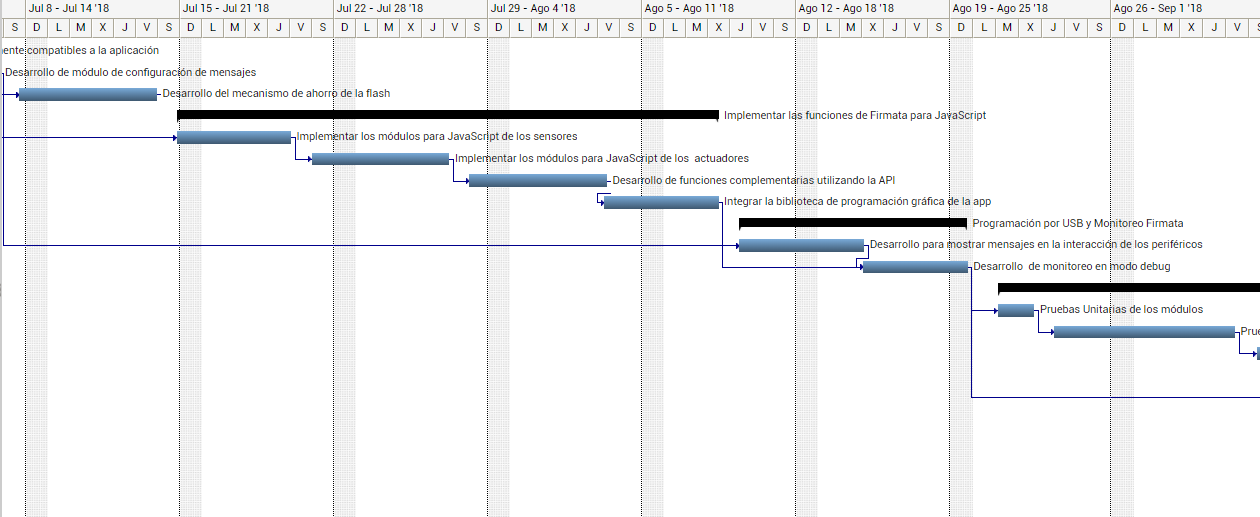
\includegraphics[scale=.30]{./Figures/diagramaGanttSegundaParte.png}
	\caption{Diagrama de Gantt - Parte 2.}
	\label{fig:diagramaGanttSegundaParte}
\end{figure}

En la figura \ref{fig:diagramaGanttTerceraParte} se puede observar la tercera parte del diagrama para este proyecto. Y la cuarta parte del diagrama se puede observar la figura \ref{fig:diagramaGanttCuartaParte} 

\begin{figure}[h]
	\centering
	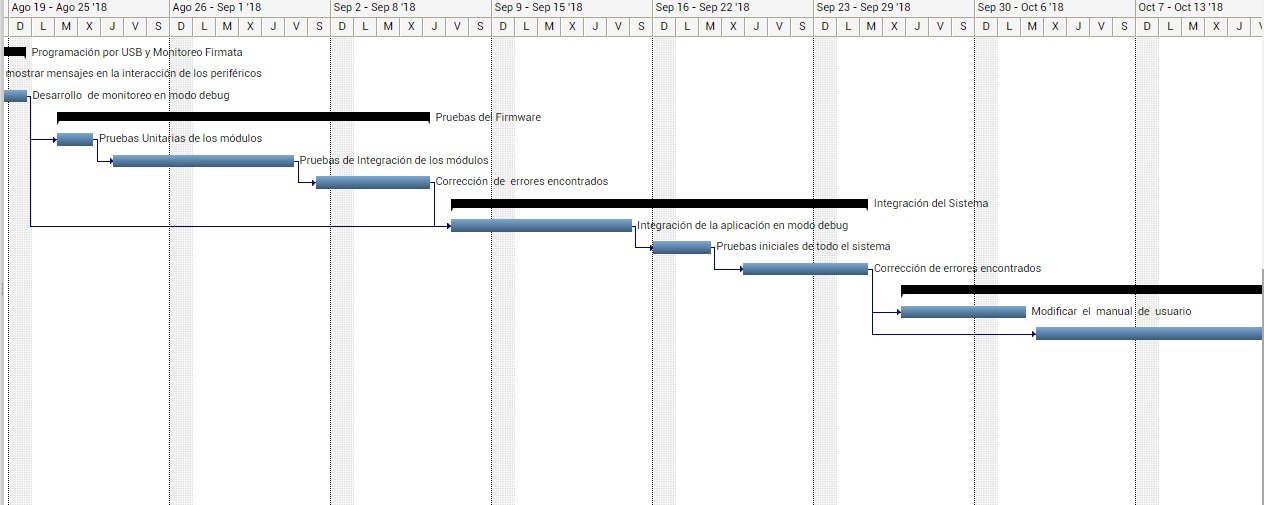
\includegraphics[scale=.30]{./Figures/diagramaGanttTerceraParte.png}
	\caption{Diagrama de Gantt - Parte 3.}
	\label{fig:diagramaGanttTerceraParte}
\end{figure}

\begin{figure}[h]
	\centering
	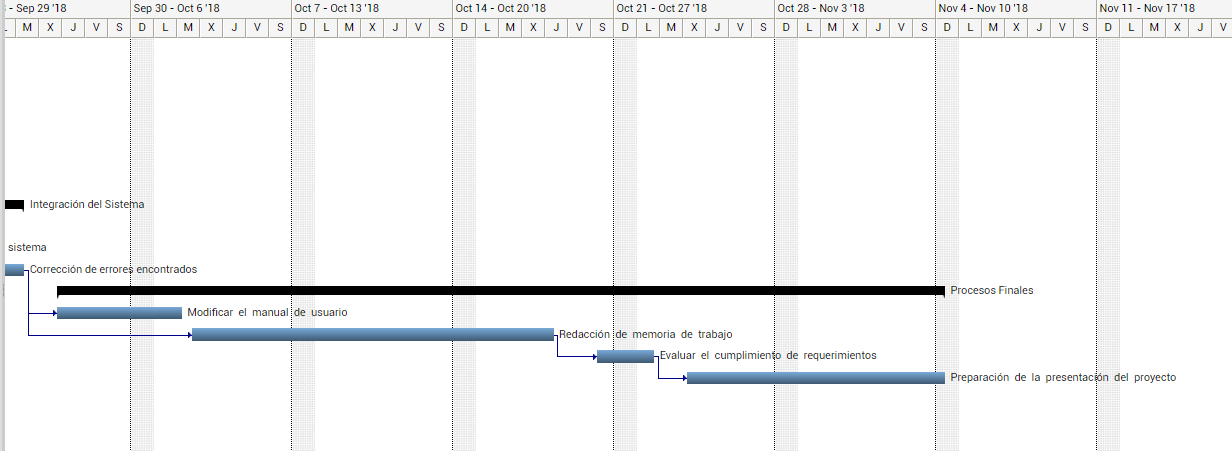
\includegraphics[scale=.30]{./Figures/diagramaGanttCuartaParte.png}
	\caption{Diagrama de Gantt - Parte 4.}
	\label{fig:diagramaGanttCuartaParte}
\end{figure}
